% !TeX root = ../../../../main.tex
% chapters/sections/chapter5/subsections/a_shock/insulation.tex

\subsection{遮断効果}
\label{sec:chapter5_a_shock_insulation_effect}
前節では外国関連主要変数が自国金融政策の影響を受けないことを確認した。
それらの外国関連主要変数は\(\beta\)ショック自体の影響は受けたが、
ここでは対照的に生産性（\(a\)）ショックの影響は受けないことをみる。
ただし、完全伸縮物価（IT-PPI）ケースについては、
遮断効果を構成する方程式系の中に価格硬直性パラメータそのものが含まれているため、
他の政策群とは異なる推移を示す点に留意が必要である。
それら外国関連変数を決定する方程式群には自国内生変数が含まれていないことを説明したが、
加えて生産性を表す変数（\(a\)）も含まれていないため\(a\)ショックの影響は受けないことになる
（付録\ref{sec:model_appendix_insulation_effect_main}を参照）。
シミュレーション結果においてもこのことを確認するため、
以下に変動する名目為替レートとこれら外国関連主要変数のグラフを表示する。
グラフ描画領域の左上に（\(10^{-15}\)）などときわめて小さな単位が書かれている場合、
グラフの変動はコンピュータによる計算誤差と考えられ、理論的には変動がないことを示している。
このことより外国関連主要変数のグラフはいずれも理論的な変動がないことがわかる。

\begin{figure}[H]
    \centering
    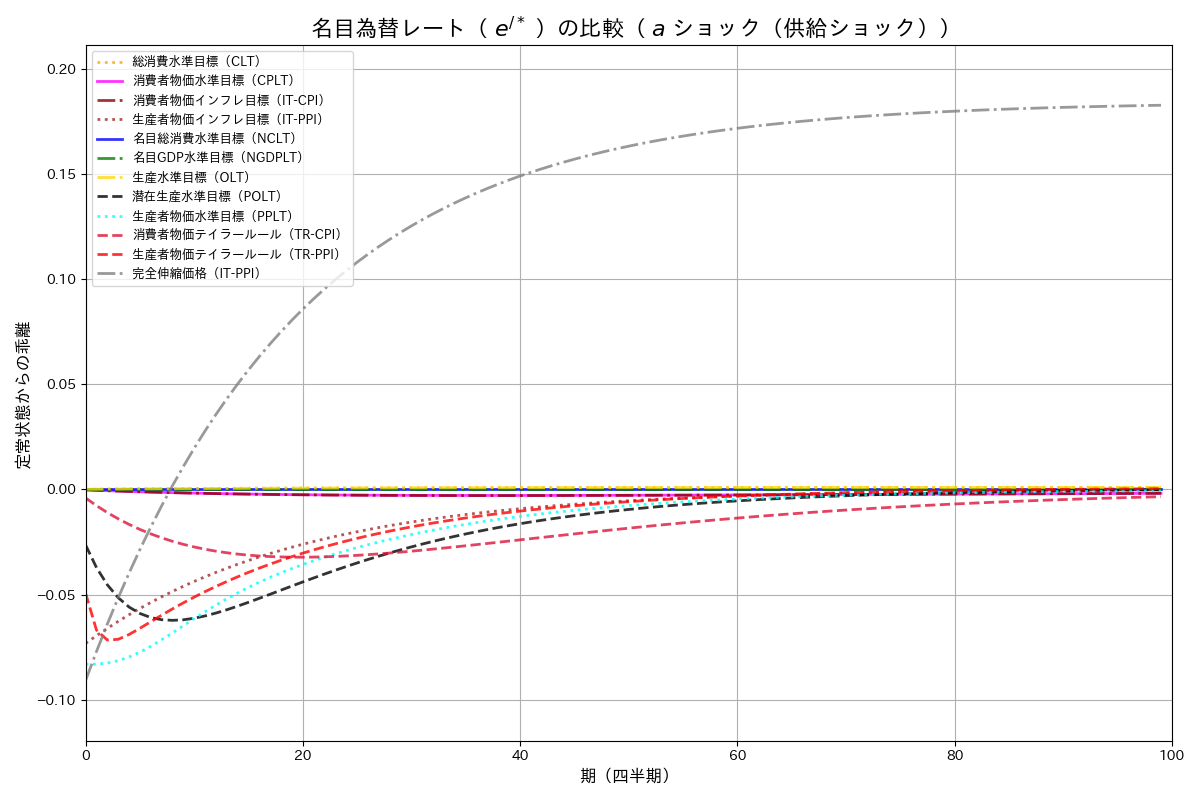
\includegraphics[width=0.9\textwidth]{comparison_graphs/a_shock/a_shock_e_slash_star.png}
    \caption{自国通貨建て名目為替レート（\(e^{/*}\)）}
    \label{fig:chapter5_a_shock_exchange_rate}
\end{figure}

\begin{figure}[H]
    \centering
    \phantomcaption % 図番号を確保
    \label{fig:chapter5_a_shock_foreign_vars}
    \makebox[\textwidth][c]{
        \begin{minipage}{1.2\textwidth}
            \centering
            \begin{subfigure}{0.48\linewidth}
                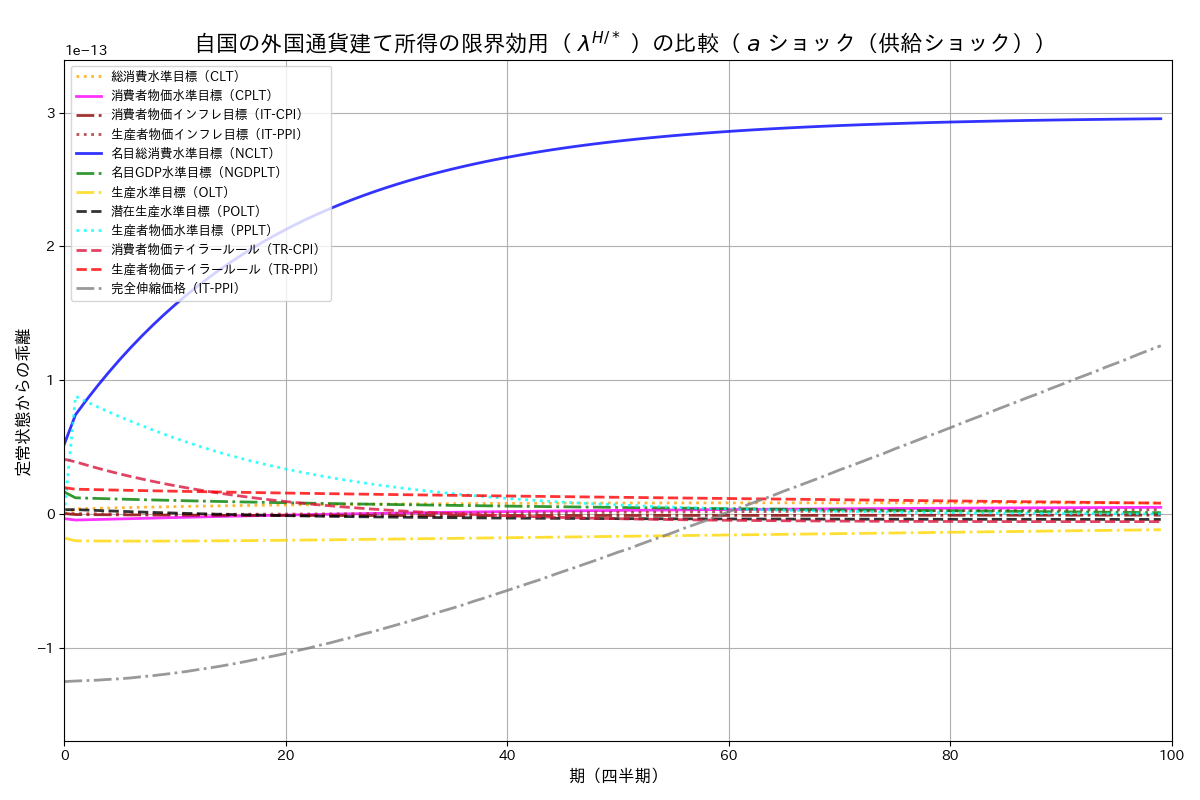
\includegraphics[width=\linewidth]{comparison_graphs/a_shock/a_shock_lambda_H_slash_star.png}
                \caption{自国の外国通貨建て所得の限界効用（\(\lambda^{H/*}\)）}
                \label{fig:chapter5_a_shock_lambda_H_slash_star}
            \end{subfigure}
            \hfill
            \begin{subfigure}{0.48\linewidth}
                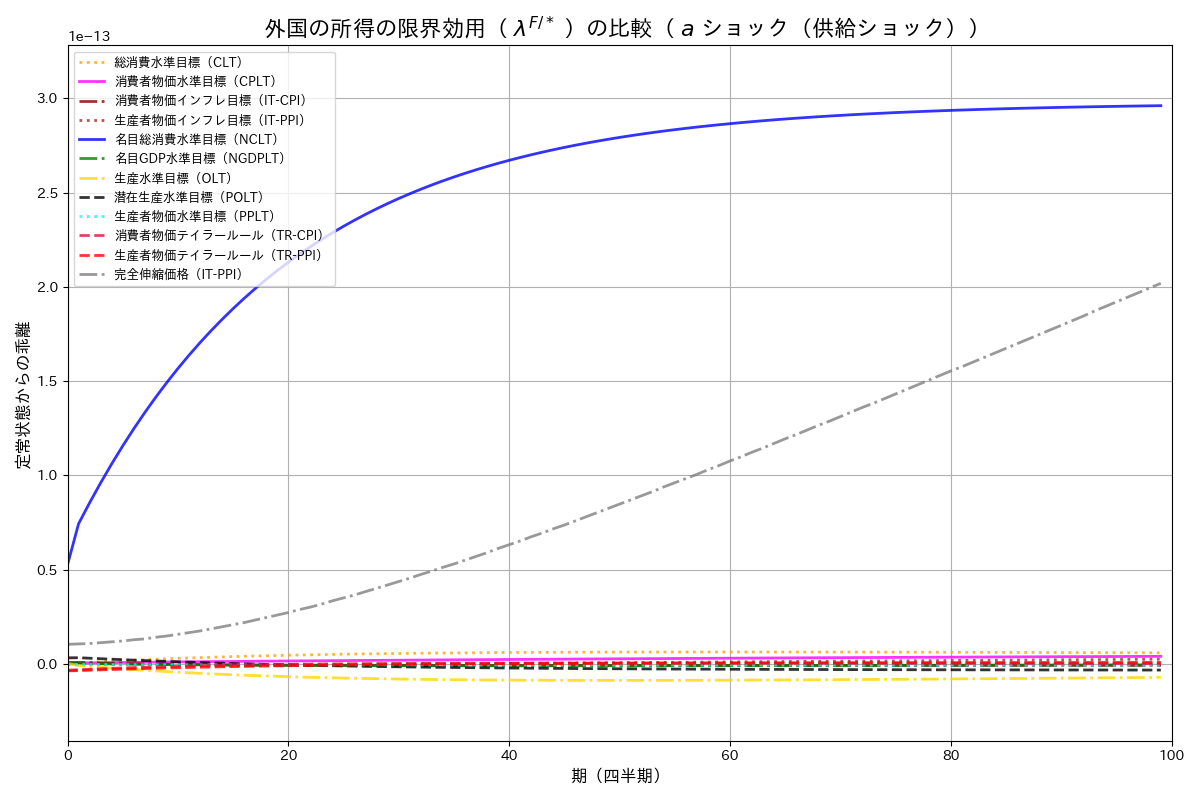
\includegraphics[width=\linewidth]{comparison_graphs/a_shock/a_shock_lambda_F_slash_star.png}
                \caption{外国の所得の限界効用（\(\lambda^{F/*}\)）}
                \label{fig:chapter5_a_shock_lambda_F_slash_star}
            \end{subfigure}
        \end{minipage}
    }
\end{figure}

\begin{figure}[H]
    \ContinuedFloat
    \centering
    \makebox[\textwidth][c]{
        \begin{minipage}{1.2\textwidth}
            \centering
            \begin{subfigure}{0.48\linewidth}
                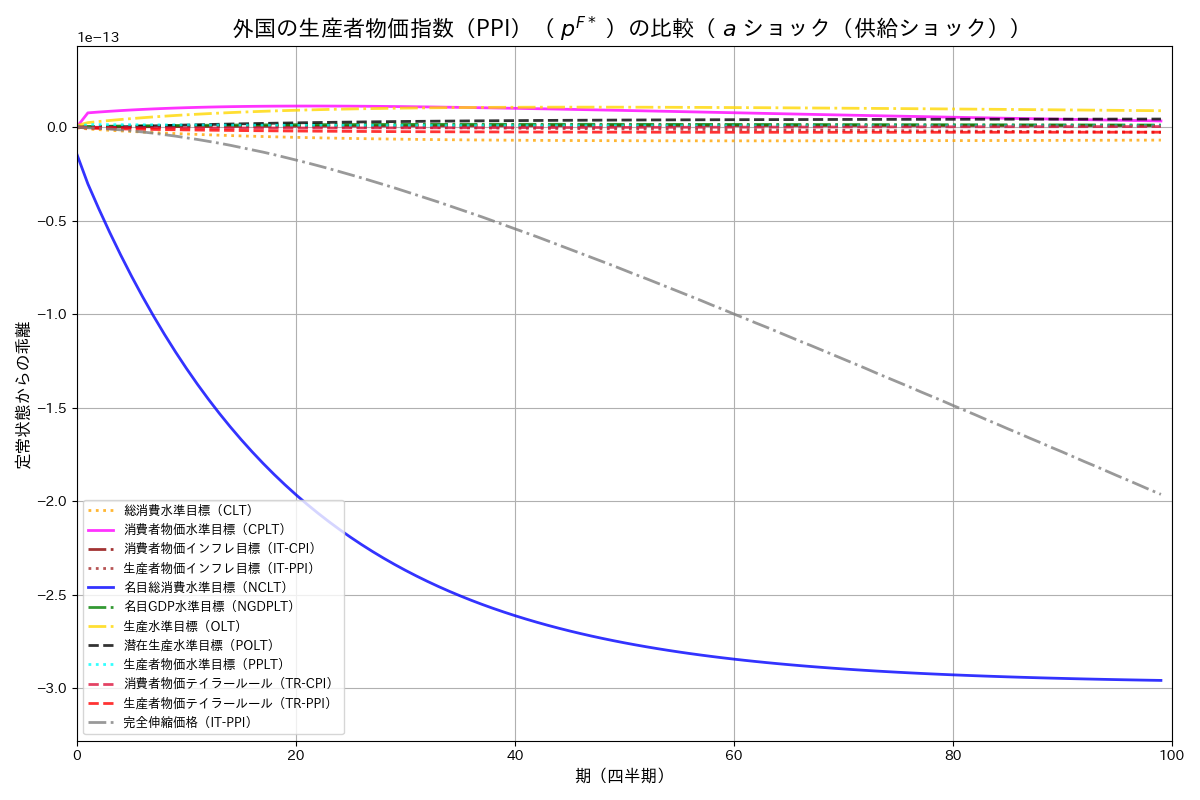
\includegraphics[width=\linewidth]{comparison_graphs/a_shock/a_shock_p_F_star.png}
                \caption{外国の生産者物価指数（PPI）（\(p^{F*}\)）}
                \label{fig:chapter5_a_shock_p_F_star_sub}
            \end{subfigure}
            \hfill
            \begin{subfigure}{0.48\linewidth}
                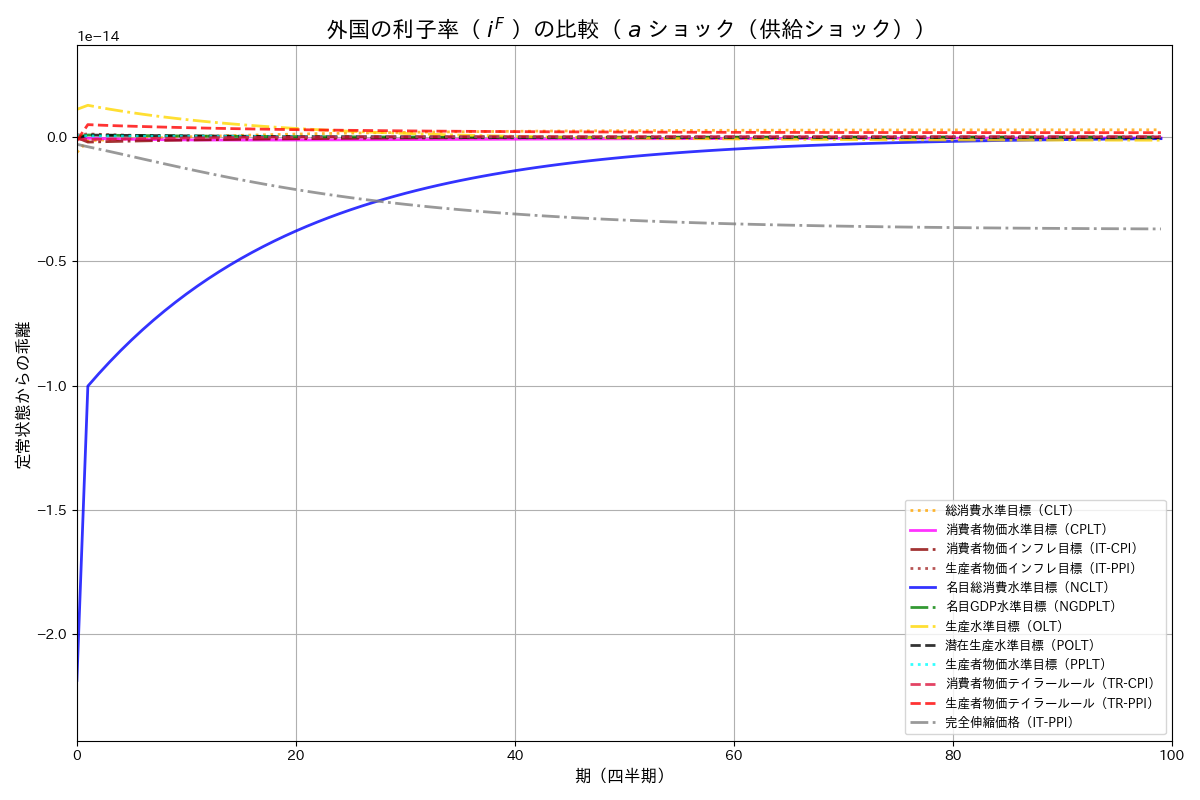
\includegraphics[width=\linewidth]{comparison_graphs/a_shock/a_shock_i_F.png}
                \caption{外国の名目利子率（\(i^F\)）}
                \label{fig:chapter5_a_shock_i_F_sub}
            \end{subfigure}
        \end{minipage}
    }
\end{figure}

\begin{figure}[H]
    \ContinuedFloat
    \centering
    \makebox[\textwidth][c]{
        \begin{minipage}{1.2\textwidth}
            \centering
            \begin{subfigure}{0.48\linewidth}
                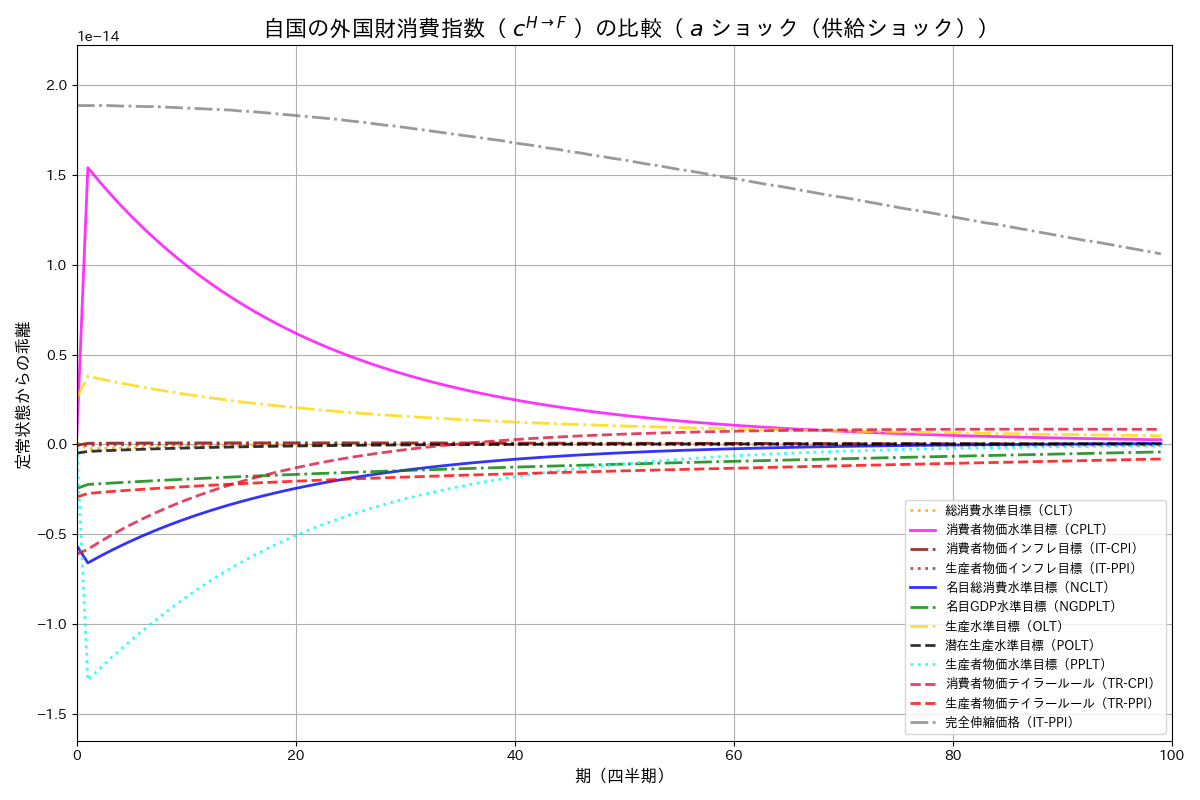
\includegraphics[width=\linewidth]{comparison_graphs/a_shock/a_shock_c_H_F.png}
                \caption{自国の外国財消費指数（\(c^{H\to F}\)）}
                \label{fig:chapter5_a_shock_c_H_F_sub}
            \end{subfigure}
            \hfill
            \begin{subfigure}{0.48\linewidth}
                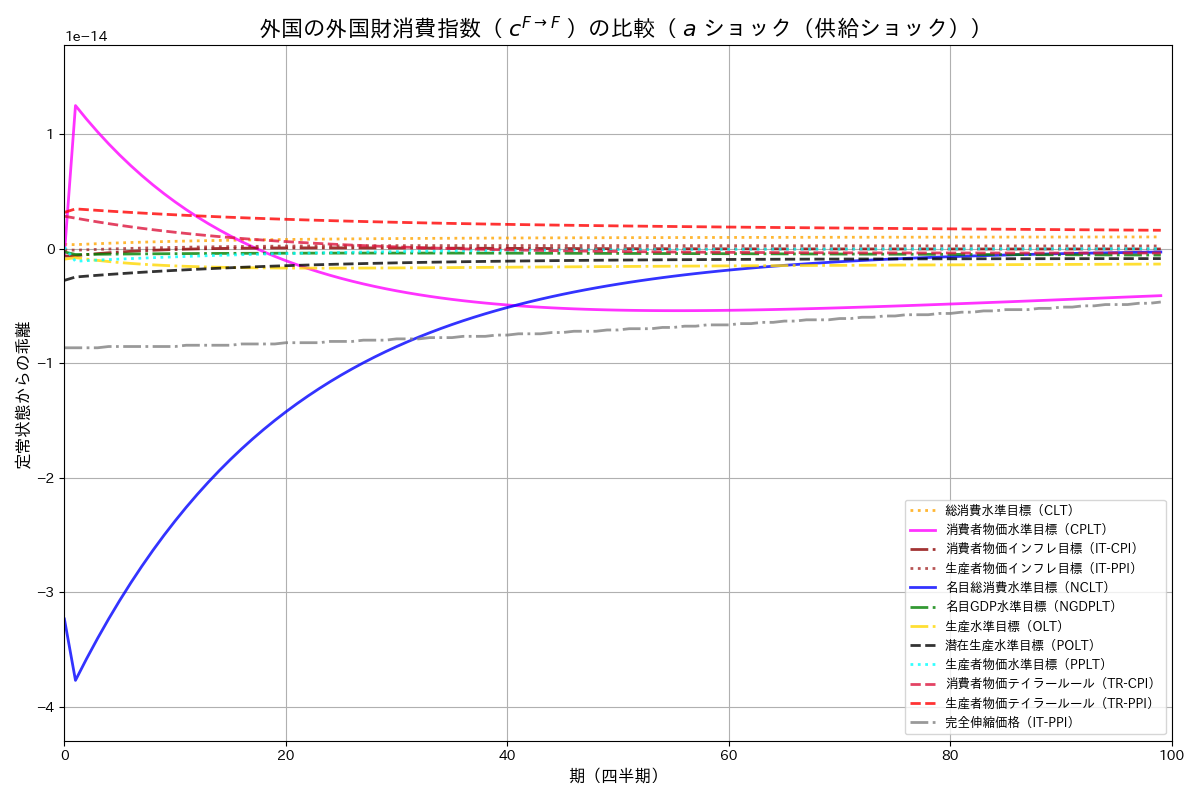
\includegraphics[width=\linewidth]{comparison_graphs/a_shock/a_shock_c_F_F.png}
                \caption{外国の外国財消費指数（\(c^{F\to F}\)）}
                \label{fig:chapter5_a_shock_c_F_F_sub}
            \end{subfigure}
        \end{minipage}
    }
\end{figure}

\begin{figure}[H]
    \ContinuedFloat
    \centering
    \makebox[\textwidth][c]{
        \begin{minipage}{1.2\textwidth}
            \centering
            \begin{subfigure}{0.48\linewidth}
                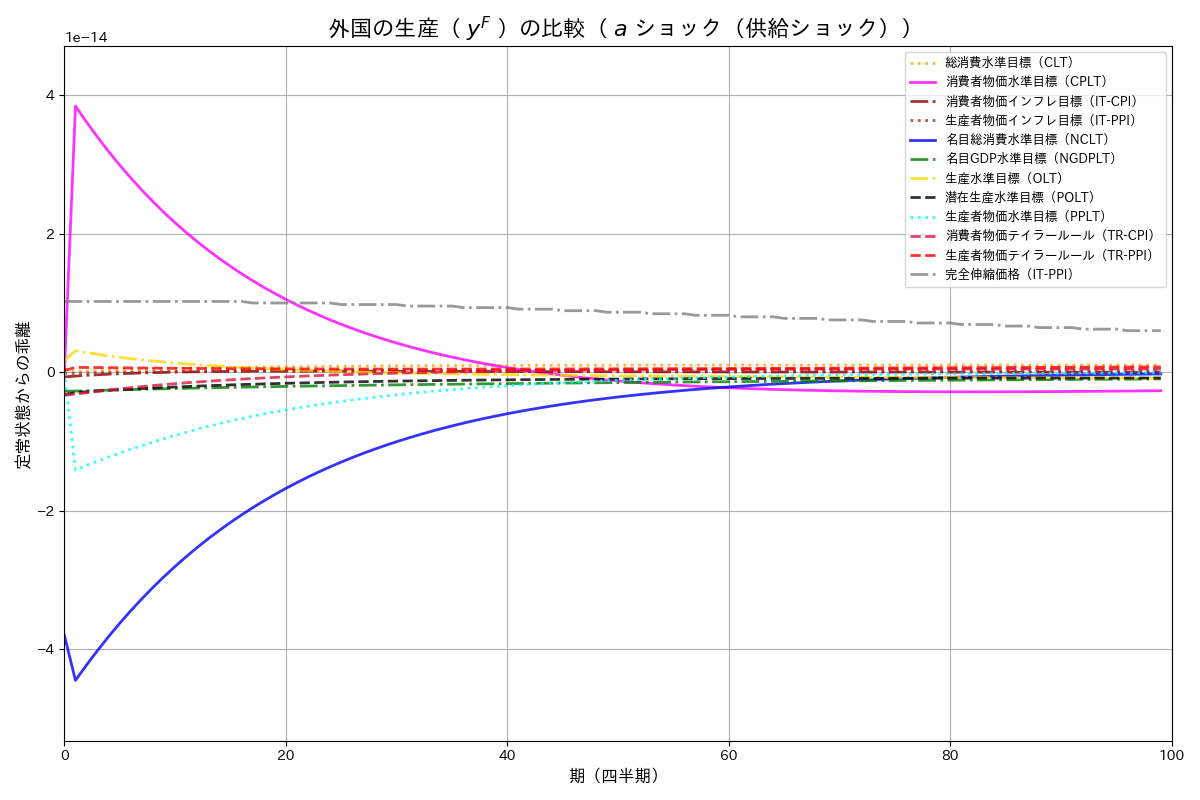
\includegraphics[width=\linewidth]{comparison_graphs/a_shock/a_shock_y_F.png}
                \caption{外国の生産（\(y^F\)）}
                \label{fig:chapter5_a_shock_y_F_sub}
            \end{subfigure}
            \hfill
            \begin{subfigure}{0.48\linewidth}
                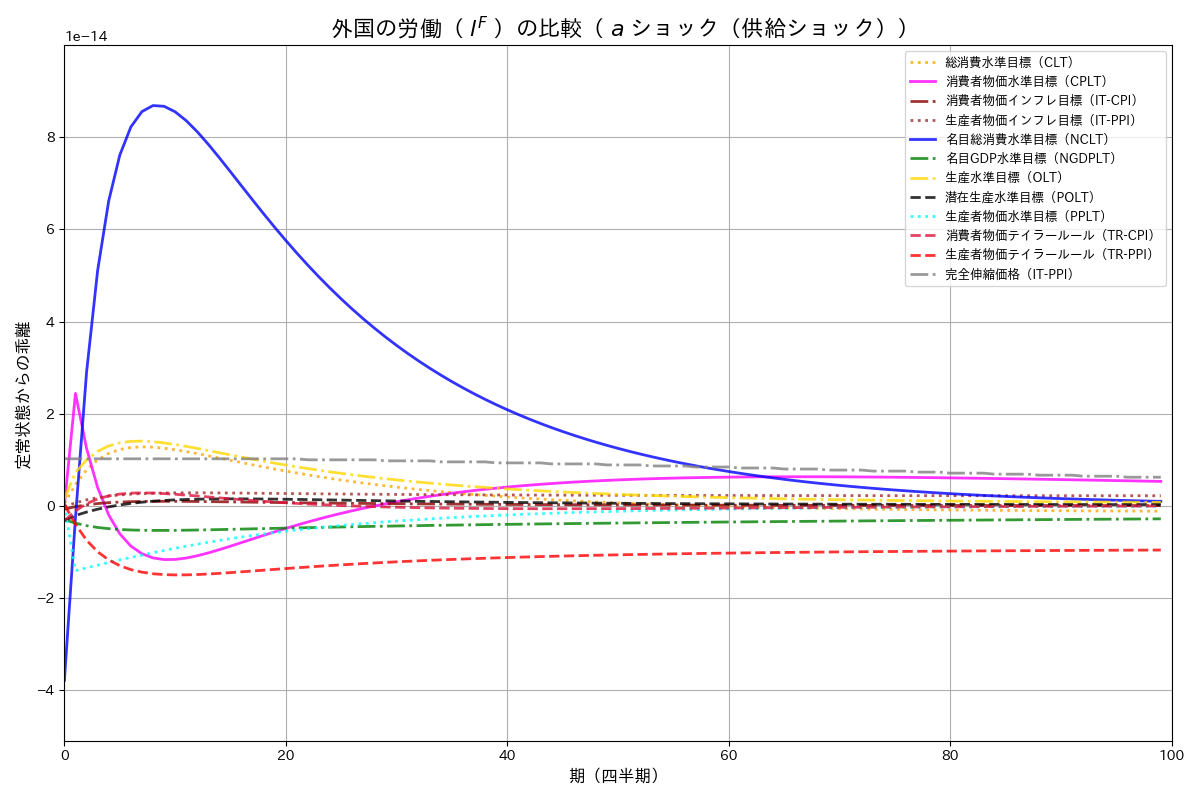
\includegraphics[width=\linewidth]{comparison_graphs/a_shock/a_shock_l_F.png}
                \caption{外国の労働（\(l^F\)）}
                \label{fig:chapter5_a_shock_l_F_sub}
            \end{subfigure}
        \end{minipage}
    }
\end{figure}

\begin{figure}[H]
    \ContinuedFloat
    \centering
    \makebox[\textwidth][c]{
        \begin{minipage}{1.2\textwidth}
            \centering
            \begin{subfigure}{0.48\linewidth}
                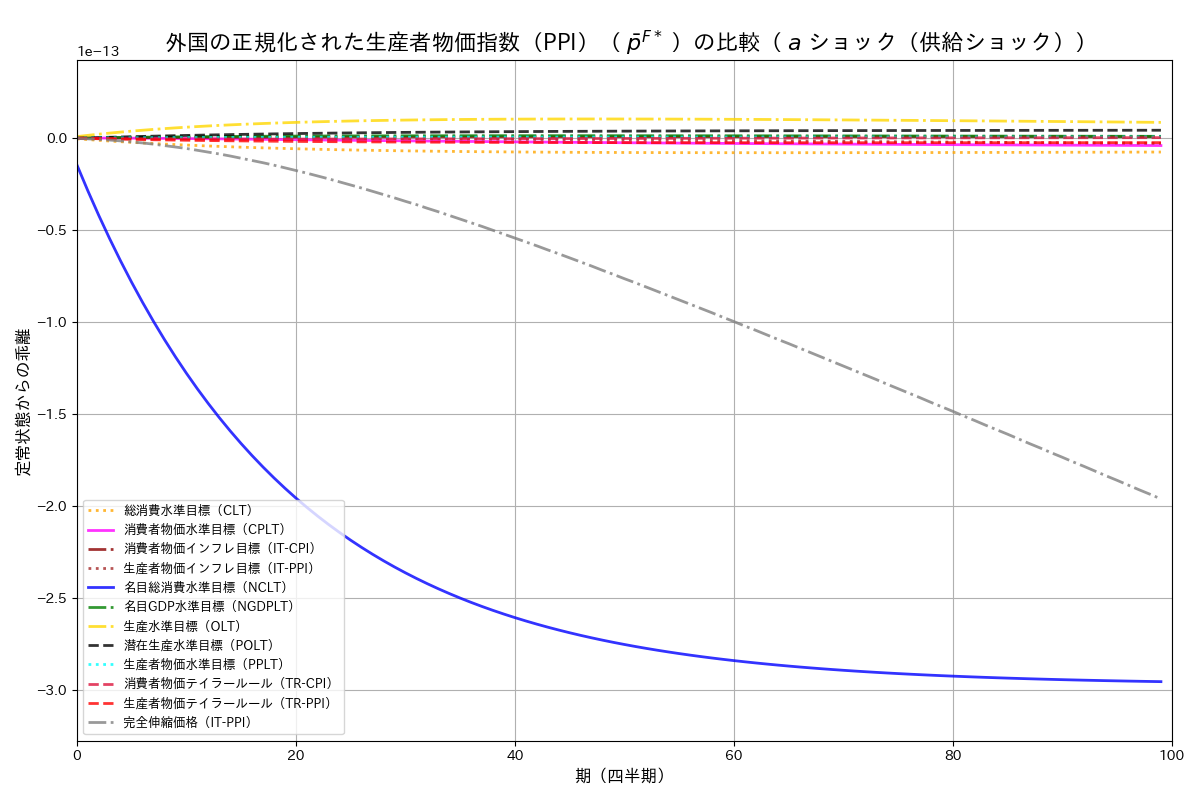
\includegraphics[width=\linewidth]{comparison_graphs/a_shock/a_shock_p_F_star_bar.png}
                \caption{外国の正規化された生産者物価指数（PPI）（\(\bar{p}^{F*}\)）}
                \label{fig:chapter5_a_shock_p_F_star_bar_sub}
            \end{subfigure}
            \hfill
            \begin{subfigure}{0.48\linewidth}
                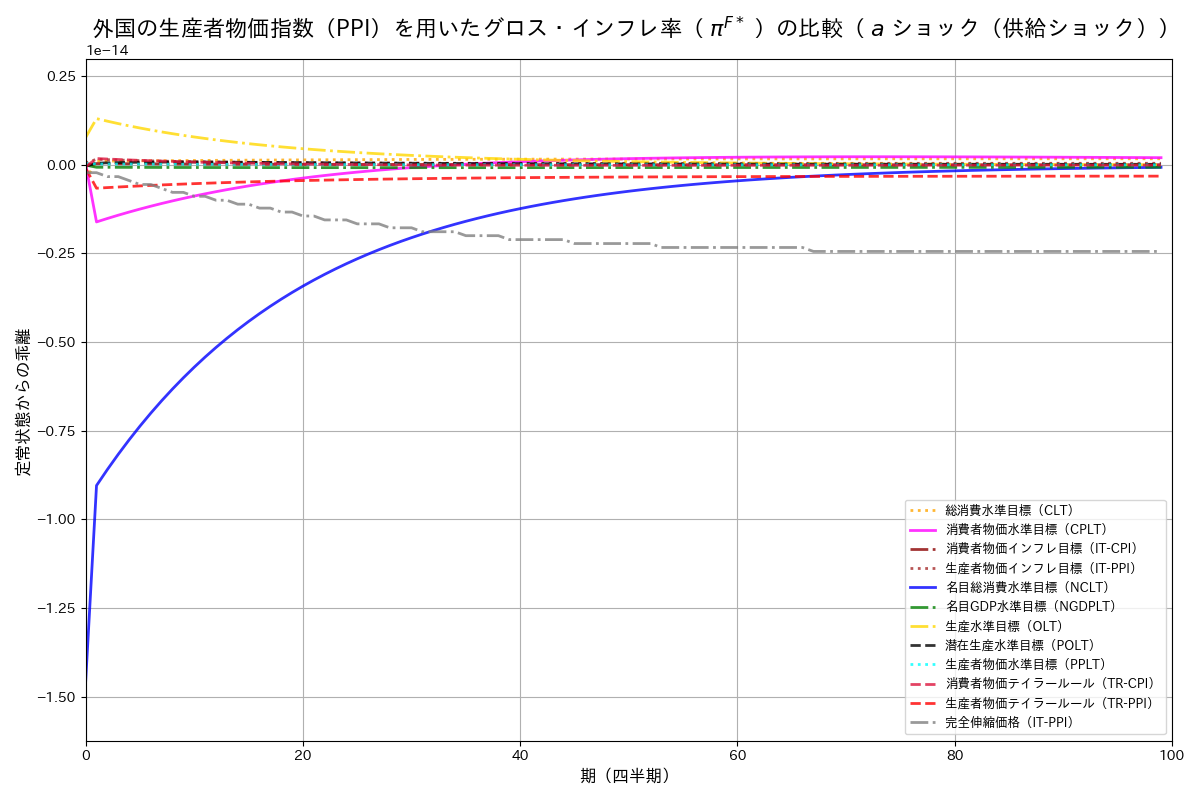
\includegraphics[width=\linewidth]{comparison_graphs/a_shock/a_shock_pi_F_star.png}
                \caption{外国の正規化された生産者物価指数を用いたグロス・インフレ率（\(\pi^{F*}\)）}
                \label{fig:chapter5_a_shock_pi_F_star_sub}
            \end{subfigure}
        \end{minipage}
    }
\end{figure}

\begin{figure}[H]
    \ContinuedFloat
    \centering
    \makebox[\textwidth][c]{
        \begin{minipage}{1.2\textwidth}
            \centering
            \begin{subfigure}{0.48\linewidth}
                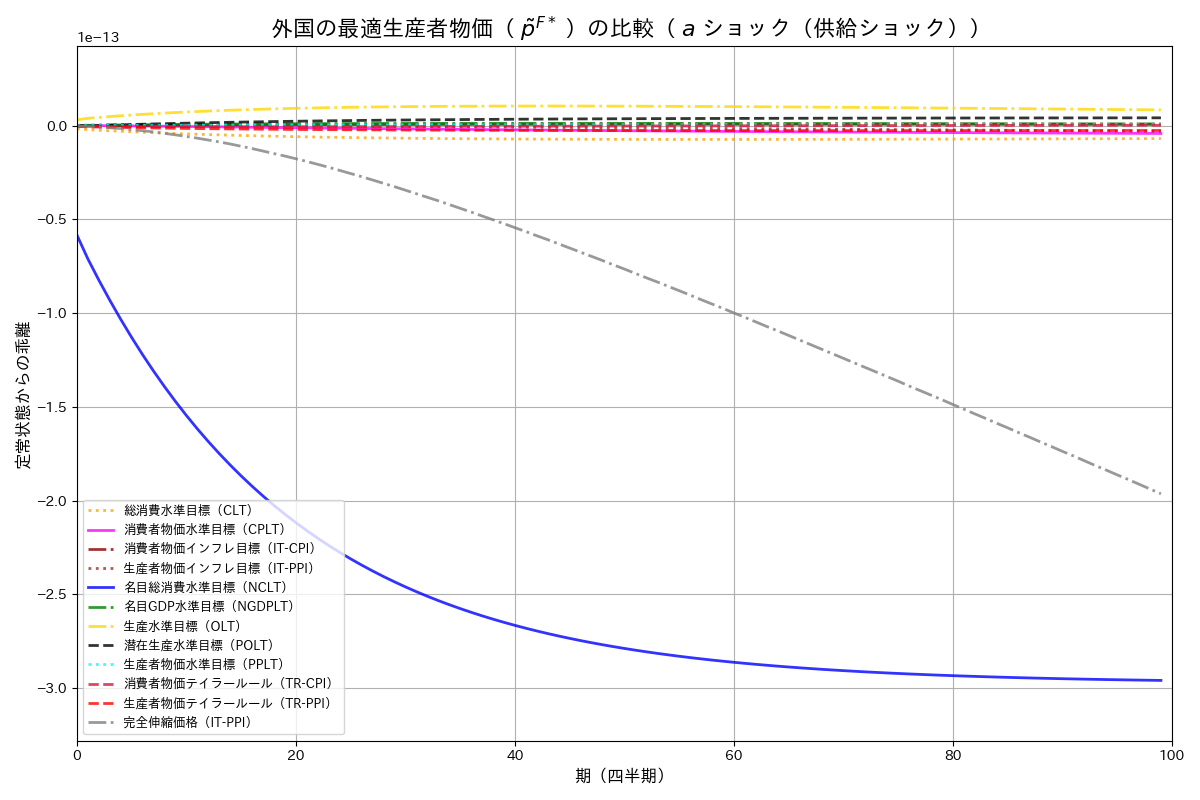
\includegraphics[width=\linewidth]{comparison_graphs/a_shock/a_shock_p_F_star_tilde.png}
                \caption{外国の最適生産者物価（\(\widetilde{p}^{F*}\)）}
                \label{fig:chapter5_a_shock_p_F_star_tilde_sub}
            \end{subfigure}
            \hfill
            \begin{subfigure}{0.48\linewidth}
                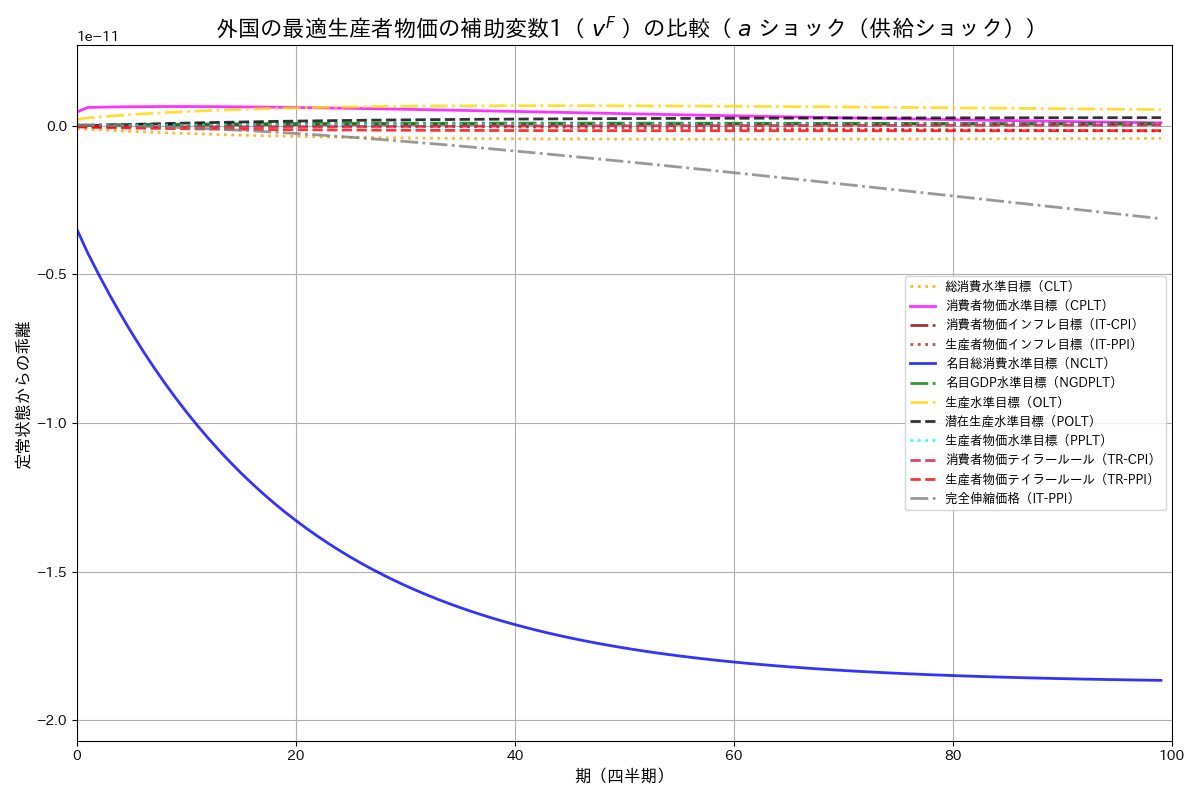
\includegraphics[width=\linewidth]{comparison_graphs/a_shock/a_shock_v_F.png}
                \caption{外国の最適生産者物価の補助変数1（\(v^F\)）}
                \label{fig:chapter5_a_shock_v_F_sub}
            \end{subfigure}
        \end{minipage}
    }
\end{figure}

\begin{figure}[H]
    \ContinuedFloat
    \centering
    \makebox[\textwidth][c]{
        \begin{minipage}{1.2\textwidth}
            \centering
            \begin{subfigure}{0.48\linewidth}
                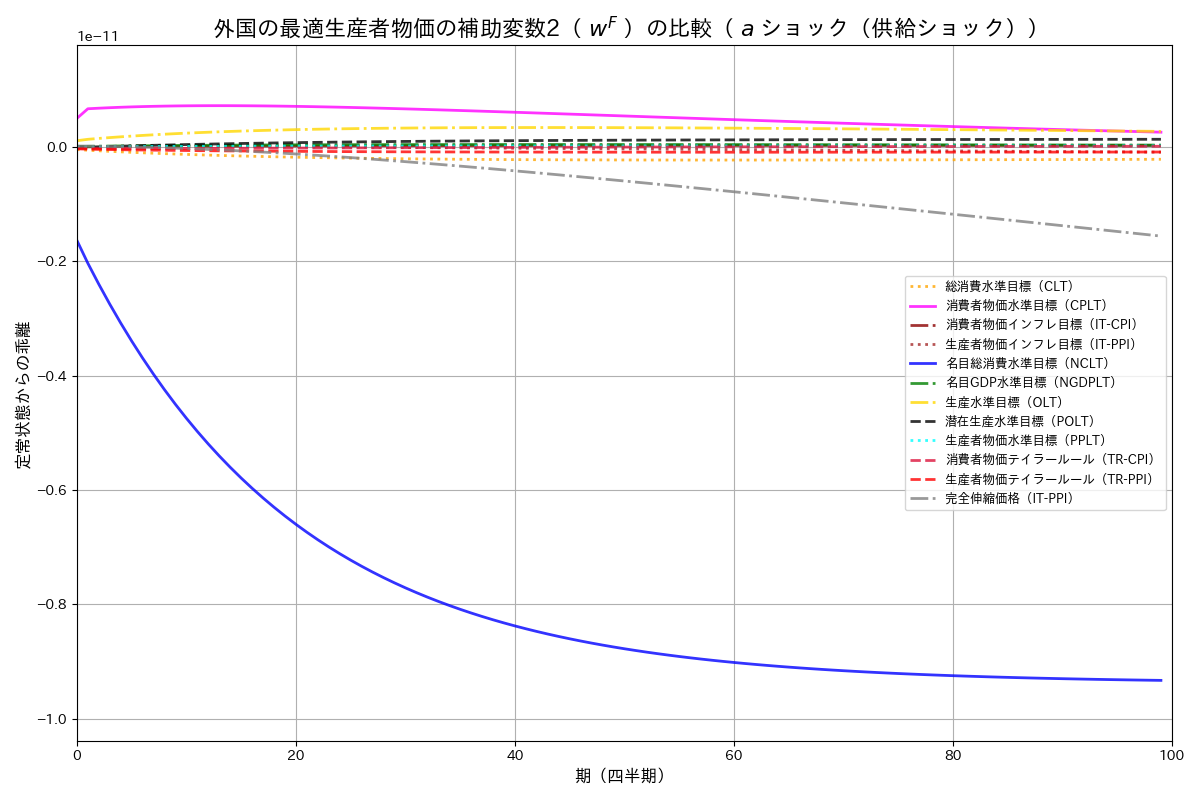
\includegraphics[width=\linewidth]{comparison_graphs/a_shock/a_shock_w_F.png}
                \caption{外国の最適生産者物価の補助変数2（\(w^F\)）}
                \label{fig:chapter5_a_shock_w_F_sub}
            \end{subfigure}
            \hfill
            \begin{subfigure}{0.48\linewidth}
                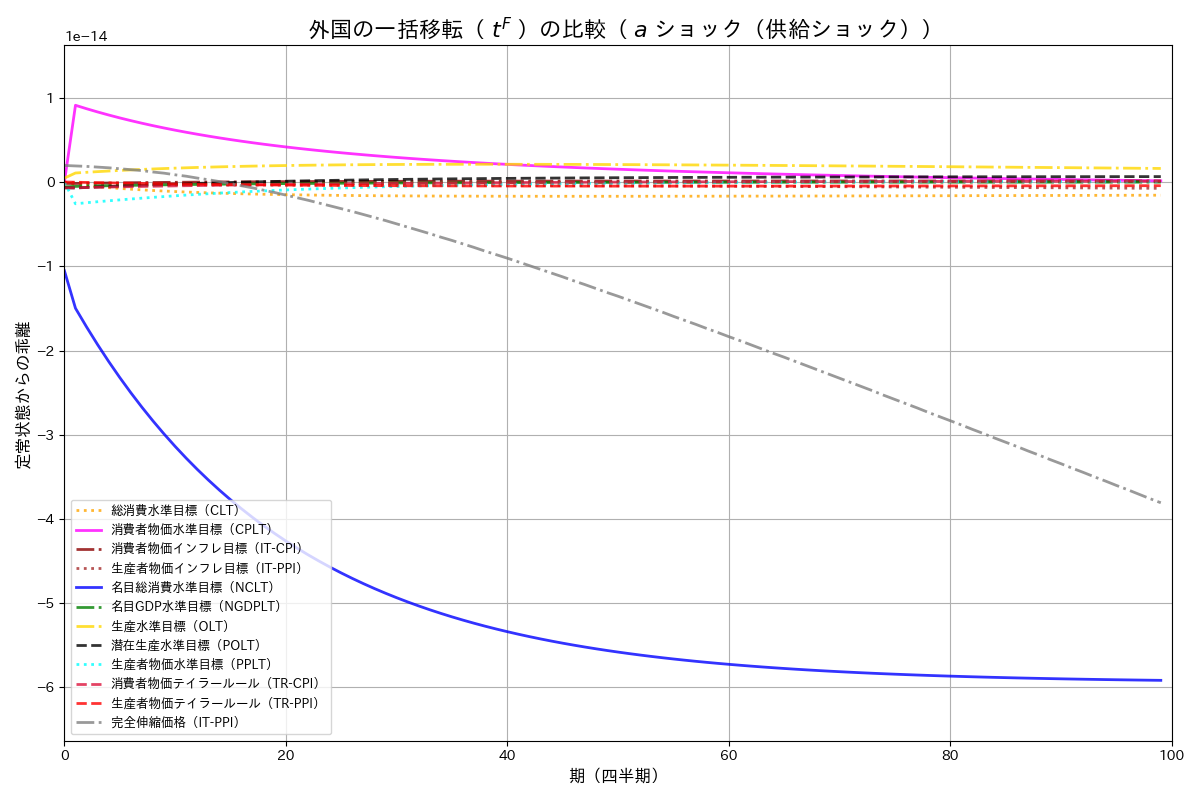
\includegraphics[width=\linewidth]{comparison_graphs/a_shock/a_shock_t_F.png}
                \caption{外国の一括移転（\(t^F\)）}
                \label{fig:chapter5_a_shock_t_F_sub}
            \end{subfigure}
        \end{minipage}
    }
\end{figure}

\begin{figure}[H]
    \ContinuedFloat
    \centering
    \makebox[\textwidth][c]{
        \begin{minipage}{1.2\textwidth}
            \centering
            \begin{subfigure}{0.48\linewidth}
                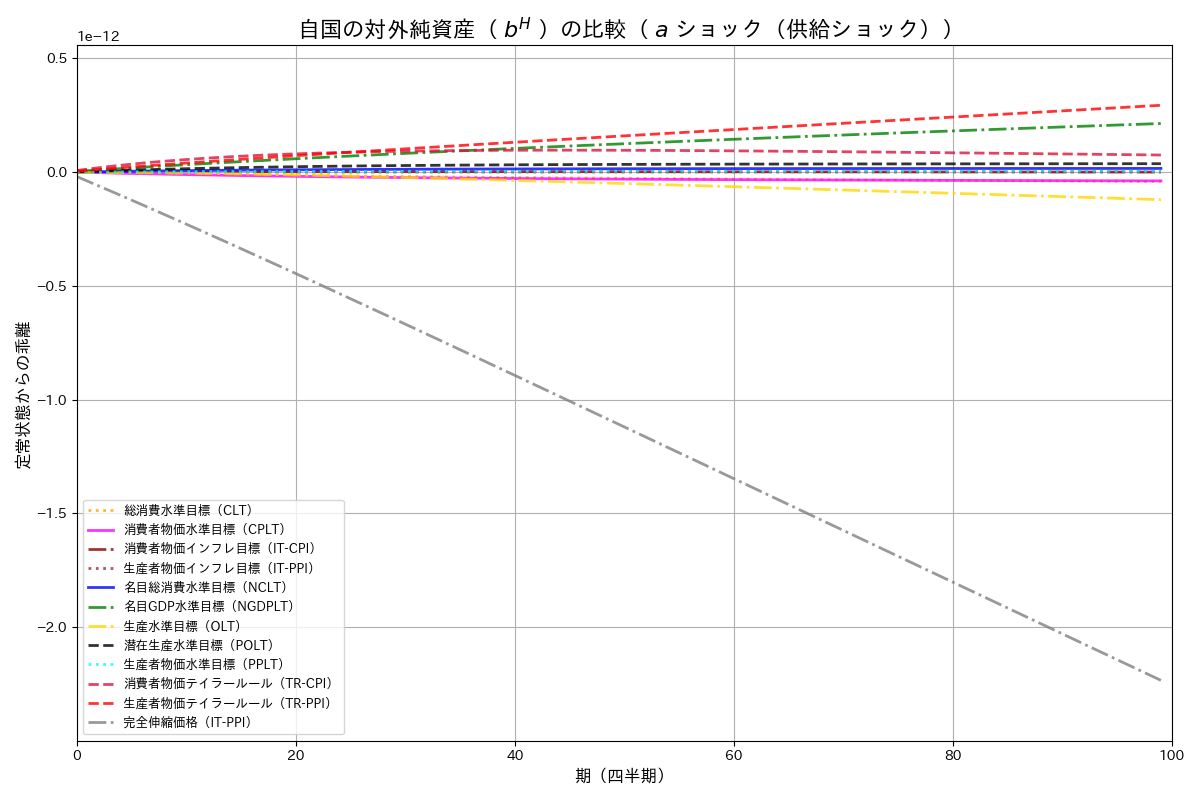
\includegraphics[width=\linewidth]{comparison_graphs/a_shock/a_shock_b_H.png}
                \caption{自国の対外純資産（\(b^H\)）}
                \label{fig:chapter5_a_shock_b_H_sub}
            \end{subfigure}
            \hfill
            \begin{subfigure}{0.48\linewidth}
                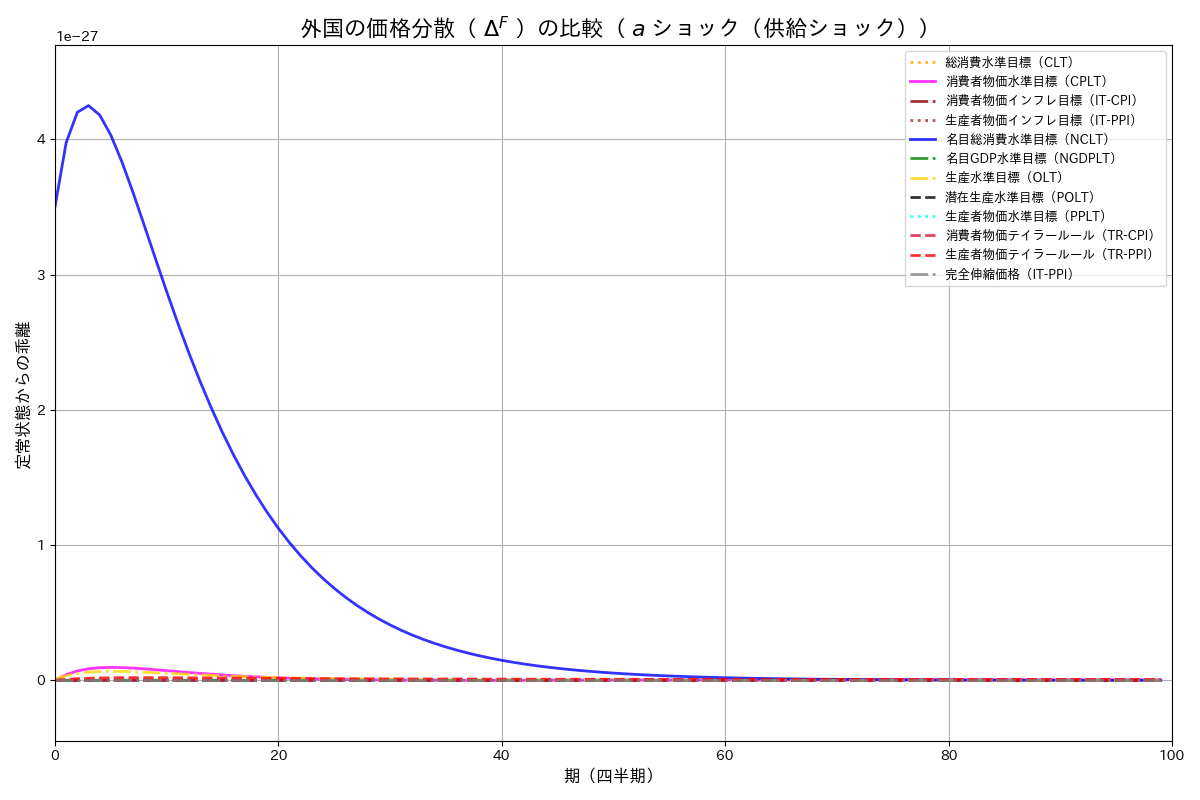
\includegraphics[width=\linewidth]{comparison_graphs/a_shock/a_shock_Delta_F.png}
                \caption{外国の価格分散（\(\Delta^F\)）}
                \label{fig:chapter5_a_shock_delta_F_sub}
            \end{subfigure}
        \end{minipage}
    }
    % 最後にまとめてキャプションを表示
    \caption{外国経済変数のインパルス応答関数（全政策で不変）}
\end{figure}
